\begin{multicols}{3}
\byline{Интервю с Лорета Добрева, 12г клас на тема DSD}{Михаела Николова, 10г клас}

% \noindent \begin{window}[2,r, 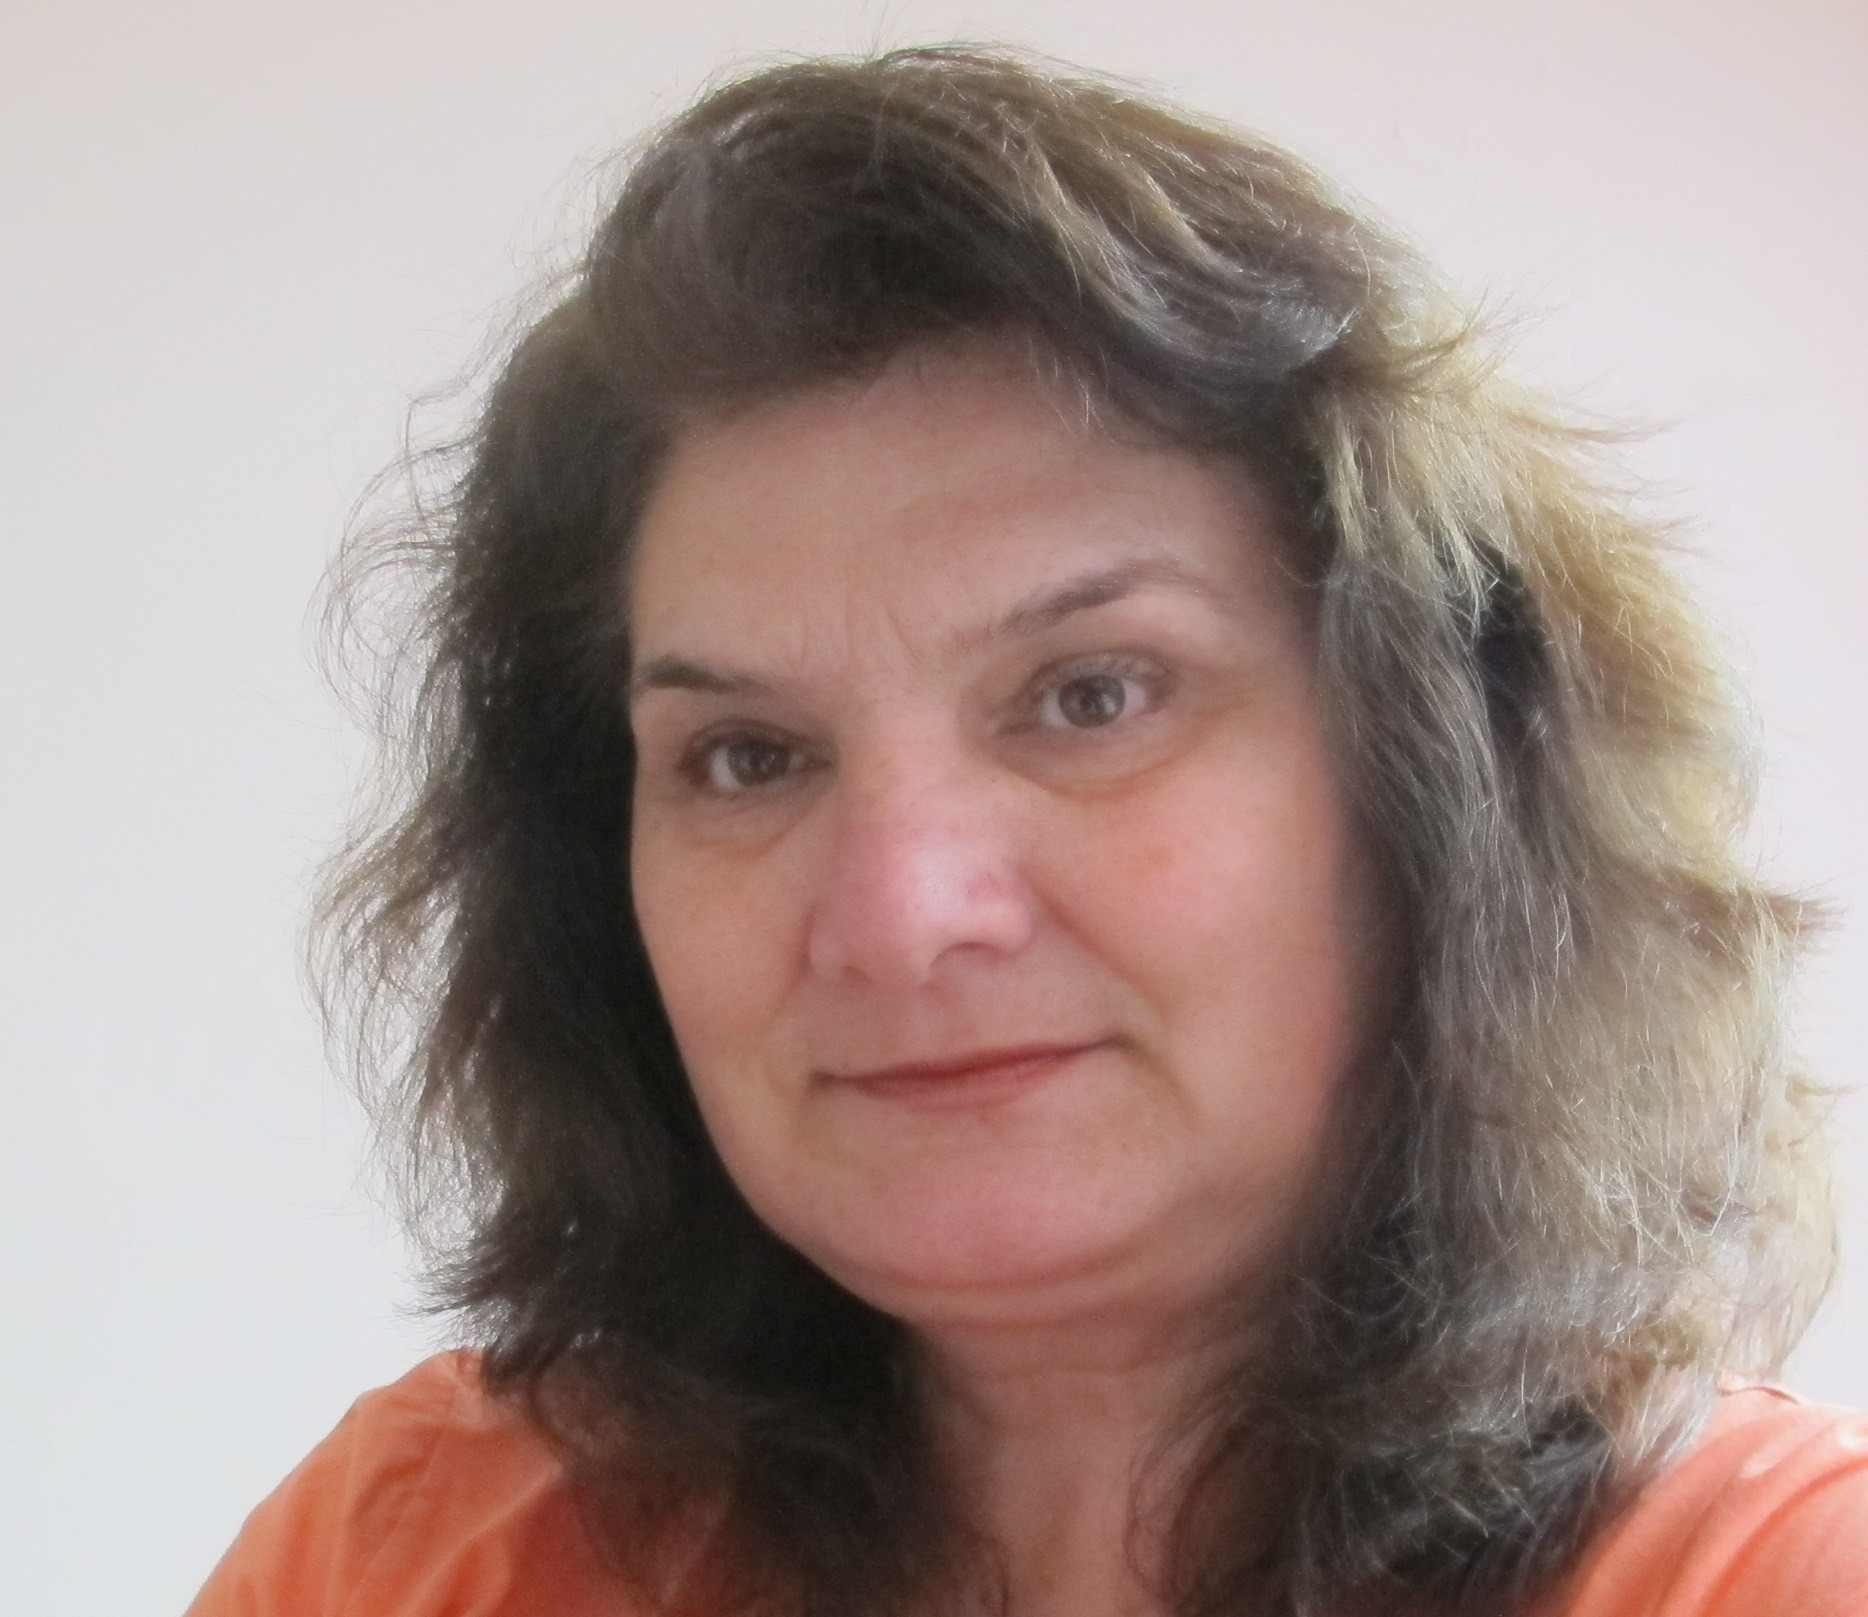
\includegraphics[width=2.1in]{./Radeva/IMG_3591.JPG},] \end{window}

Как се чувстваш след изпита, изглежда ли толкова труден след като е минал вече?

Лорета: Истината е, че в началото на 12 клас бях доста стресирана, защото знаех, че с този сертификат мога да уча в Германия, което всъщност беше и моето основно желание. Сега, след изпита, разбрах, че всички тези притеснения са били напразни, защото не е толкова страшно, колкото ни се представя и е доста по- лесно, колкото си мислим. Основното е да си постоянен и всичко ще е много по-лесно.

Как очакваше да премине всичко? 

Лорета:  Очаквах всичко да премине както съм го планувала, защото вярвах в себе си, че имам нужното ниво, за да се явя на изпита.

Притесняваше ли се?

Лорета: Притеснявах се изключително много, защото знаех, че това е една от стъпките, които ще осъществят следването ми в Германия. Разболях се ден преди писмения изпит заради притеснението ми. На устния изпит се притеснявах по-малко и дори когато влязох при изпитващите притеснението ми се изпари почти веднага.

На какво най-много трябва да се обърне внимание относно изпита?

Лорета: Абсолютно всеки един компонент е важен и нищо не трябва да се пренебрегва. Чрез постоянни упражнения нещата стават по-лесни, а и човек става по-уверен в себе си.

Можеш ли да дадеш съвети на всички, на които им предстои да се явят на изпита?

Лорета: Няма да ви давам съвет да не се притеснявате, защото това е невъзможно. Притеснението е нормално, след като този изпит отваря пътища за доста от учениците на ГПНЕ. Мога да ви посъветвам да се стараете, да четете по темите и да гледате на изпита от положителната страна, защото след това ще разберете, че това е бил правилният подход към успеха.
\closearticle
\end{multicols}
